\chapter{Especificación de requerimientos}
\section{Pila de producto}

La pila de producto contiene las funcionalidades que se desean desarrollar para el sistema “Lector de PDF Minimalista”. Estas funcionalidades se expresan mediante historias de usuario, ya que permiten describir cada requerimiento desde la perspectiva de la persona que utilizará la aplicación.

Para identificar las historias se utiliza el código US, que significa User Story. La numeración se asigna de forma consecutiva. La columna Prioridad indica la importancia de cada funcionalidad para el proyecto, mientras que la columna Inserción señala si la historia formaba parte del alcance original o si fue agregada durante el Sprint 1. En el caso de que las tareas sean originales se encontrarán en color negro, si las tareas son nuevas se encontrarán en color verde y si fueron eliminadas se encontrarán en color rojo.

La pila de producto está organizada alrededor de cuatro áreas principales:

\begin{itemize}
    \item Interfaz minimalista y gestión general de la aplicación.
    \item Visualización, navegación y búsqueda dentro de documentos PDF.
    \item Edición, combinación y organización de páginas.
    \item Funcionalidades complementarias, como el modo presentación y la navegación mediante el outline.
\end{itemize}

\subsection{Requerimientos funcionales del sistema}

% La pila del producto debe actualizarla cada iteración del proyecto. Debe documentar los cambios sufridos durante la iteración pasada, de forma que se pueda trazar con mucho detalle los cambios que ha sufrido la definición del proyecto desde sus inicios. Si durante el desarrollo cambia alguno de los MVP o la EDT, debe modificarlos también y documentar la razón que justifica el cambio.

%% PILA DE PRODUCTO %%
\begin{longtable}{|l||p{7cm}|l|l|}

\multicolumn{4}{c}{Pila general del producto}\\
\hline\hline
\textbf{Código} & \textbf{Descripción} & \textbf{Prioridad} & \textbf{Inserción}\\
\hline
\endfirsthead
\textbf{Código} & \textbf{Descripción} & \textbf{Prioridad} & \textbf{Inserción}\\
\hline\hline
\endhead

%\textbf{RFXXX} & 
%\textbf{Título de la historia:} Descripción de la funcionalidad que representa la historia, lo más detallado posible y con énfasis en la implementación de funcionalidad. & Alta & Original\\

%\color{ForestGreen}
%\textbf{RF002} & Una historia nueva en este sprint & Media & Sprint 1 \\

%\color{Mahogany}
%\textbf{RF003} & Una historia eliminada & Baja & Original \\

\textbf{US001} & 
\textbf{Aplicación de escritorio minimalista:} Como usuario, quiero una interfaz limpia y minimalista para la aplicación, de modo que pueda enfocarme en la lectura del contenido sin distracciones visuales. & Muy Alta & Original\\

\textbf{US002} & 
\textbf{Compaginar archivos PDF:} Como usuario, quiero poder compaginar múltiples documentos o páginas, para organizar la estructura del documento final de manera lógica antes de exportarlo. & Media & Original\\

\textbf{US003} & 
\textbf{Mezclar archivos PDF:} Como usuario, quiero poder intercalar o mezclar páginas de dos o más PDFs distintos, para consolidar información de múltiples fuentes en un solo archivo. & Alta & Original\\

\textbf{US004} & 
\textbf{Abrir varios archivos PDF:} Como usuario, quiero tener la capacidad de abrir dos archivos PDF simultáneamente (en pantalla dividida o pestañas), para comparar su contenido o trabajar con ambos de forma paralela. & Media & Original\\

\textbf{US005} & 
\textbf{Visualización ajustada al pdf:} Como usuario, quiero que la aplicación renderice y adapte correctamente la visualización del documento al tamaño de mi ventana con la función de prioridad en pantalla, para una experiencia ergonómica y de uso sobre otras aplicaciones. & Media & Original\\

\textbf{US006} & 
\textbf{Presentar PDF:} Como usuario, quiero activar un modo de presentación a pantalla completa, para poder exponer el contenido del documento a una audiencia ocultando los menús y herramientas. & Media & Original\\

\textbf{US007} & 
\textbf{Eliminar páginas de un PDF:} Como usuario, quiero poder seleccionar y eliminar páginas específicas de un PDF, para remover información irrelevante o incorrecta del documento original. & Media & Original\\

\textbf{US008} & 
\textbf{Guardar un PDF:} Como usuario, quiero poder guardar los cambios realizados sobre el archivo PDF actual, para asegurar y no perder el progreso de mi edición. & Media & Original\\

\textbf{US009} & 
\textbf{Reordenar páginas de un PDF:} Como usuario, quiero poder reordenar las páginas del documento (por ejemplo, arrastrándolas), para ajustar el flujo de lectura y la organización según mis necesidades. & Media & Original\\

\textbf{US010} & 
\textbf{Outline del PDF:} Como usuario, quiero visualizar el índice (outline) del documento en un panel lateral, para comprender rápidamente la jerarquía y estructura general del texto. & Media & Original\\

\textbf{US011} & 
\textbf{Navegar Outline:} Como usuario, quiero poder hacer clic en cualquier sección del índice (outline) y saltar directamente a esa página, para navegar ágilmente a través de documentos muy extensos. & Media & Original\\

\textbf{US012} & 
\textbf{Guardar nuevo PDF:} Como usuario, quiero tener la opción de "Guardar como" para generar un nuevo archivo con mis modificaciones, manteniendo el PDF original intacto como respaldo. & Media & Original\\

\textbf{US013} & 
\textbf{Buscar Texto:} Como usuario, quiero utilizar una barra de búsqueda para encontrar palabras o frases específicas dentro del documento, para localizar datos puntuales sin tener que leer todo el texto. & Media & Original\\

\textbf{US014} & 
\textbf{Abrir un PDF:} Como usuario, quiero poder abrir un archivo PDF desde el explorador de archivos de mi dispositivo, para acceder a su contenido dentro de la aplicación. & Muy Alta & Original\\

\textbf{US015} & 
\textbf{Ver páginas de un PDF:} Como usuario, quiero poder visualizar las páginas individuales del documento, para poder consumir la información que contienen. & Media & Original\\

\textbf{US016} & 
\textbf{Copiar texto portapapeles:} Como usuario, quiero poder copiar el texto previamente seleccionado al portapapeles del sistema, para pegarlo y reutilizarlo en otras herramientas o correos. & Media & Original\\

\textbf{US017} & 
\textbf{Zoom de un PDF} Como usuario, quiero poder acercar (zoom in) y alejar (zoom out) la vista de la página, para visualizar detalles pequeños o evaluar la distribución completa de la hoja. & Media & Original\\

\textbf{US018} & 
\textbf{Scroll de un PDF:} Como usuario, quiero poder desplazarme verticalmente (scroll) a lo largo del documento, para mantener una experiencia de lectura continua y fluida. & Media & Original\\

\textbf{US019} & 
\textbf{Seleccionar texto:} Como usuario, quiero poder seleccionar bloques de texto arrastrando el cursor, como acción indispensable antes de poder copiar o resaltar el contenido. & Media & Original\\

\textbf{US020} & 
\textbf{Saltar a Página:} Como usuario, quiero poder ingresar un número específico de página, para saltar a esta inmediatamente sin tener que scrollear & Media & Original\\

\textbf{US021} & 
\textbf{Mostrar Conteo de Páginas:} Como usuario, quiero poder la página en la que estoy en relación a la cantidad total de páginas, para saber con certeza en que parte del documento me encuentro. & Media & Original\\

\textbf{US022} & 
\textbf{Menú Click Derecho:} Como usuario, quiero poder mostrar un menú con click derecho, para acceder a todas las funcionalidades del sistema sin que estas se entrometan en el lector. & Media & Original\\
\hline


\caption{\color{ForestGreen}VERDE: Historias agregadas en esta iteración. \color{Mahogany}ROJO: Historias eliminadas.}
\label{ProductBacklog}

\end{longtable}

\subsection{Bitácora de cambios}

%Documente en esta sección las decisiones que llevaron a la creación de nuevas historias, o la eliminación de historias ya analizadas. Detalle con cuidado todas las historias afectadas con su respectivo código, indicando por qué razón fue eliminada / agregadas a la pila.

%Se añadieron las historias de usuario US-020 y US-021 ya que, al iniciar la implementación se determinó que sería ideal contar con la opción de visualizar el número de página actual y ofrecer la opción de saltar a una página específica sin necesidad de iterar por todas las demás mediante el scroll, de modo que, aunque la página sea de estilo minimalista, ofrezca facilidad de movimiento y visualización del archivo PDF.

Durante el desarrollo del sprint fue necesario agregar algunas correcciones denotadas con el código FX-\#\#\#\#, y dos tareas con el código TK-\#\#\#\#, esto para llevar un buen orden de desarrollo y asegurar el correcto funcionamiento de la aplicación al unir funcionalidades. Estas fueron las siguientes:
\begin{itemize}
    \item FX-001: Presentar toma URL en vez de PDF.
    \item FX-002: Unir Viewer y PresentationViewer con OpenFile.
    \item FX-003: Unir Zoom con Viewer
    \item FX-004: Refactorizar código para que esté en línea con el estándar.
    \item TK-001: Definir estándar de código.
    \item TK-002: Investigación preliminar sobre la implementación de GAUDI.
\end{itemize}

\section{Producto Mínimo Viable de la iteración X}

El primer prototipo será una aplicación de escritorio para Windows con una interfaz sencilla y minimalista, pensada para que el usuario pueda concentrarse en la lectura sin tener demasiados botones o herramientas visibles. Contará con un menú lateral para consultar el outline del documento y un menú contextual accesible mediante clic derecho. La aplicación permitirá abrir archivos PDF, visualizarlos de forma continua, desplazarse entre sus páginas, consultar la página actual y el total de páginas, saltar directamente a una página específica, buscar palabras o frases, seleccionar y copiar texto, ajustar el zoom y adaptar el documento al tamaño de la ventana.

Además, el usuario podrá guardar el PDF actual o crear una copia mediante la opción “Guardar como”. También podrá eliminar y reordenar páginas, abrir más de un documento al mismo tiempo y combinar varios archivos PDF en uno solo. Antes de guardar el documento combinado, se mostrará una vista previa para comprobar el resultado. Finalmente, el prototipo incluirá un modo de presentación en pantalla completa, pensado para mostrar el contenido de una página a la vez durante una exposición. Esta primera versión servirá como base para agregar en los siguientes sprints las anotaciones, los comentarios, la firma digital y el soporte para formatos como EPUB, DVI y Markdown.

\subsection{Pila de trabajo de la iteración X}

%Describa la capacidad instalada de su equipo de trabajo, incorpore información que describa, para esta iteración, cuál es el presupuesto disponible en puntos de historia. Indique también si algún miembro del equipo tiene un rol especializado y cuántas horas le dedicará al rol respectivo.
El presupuesto disponible en puntos de historia es de 72 puntos como se muestra en el cuadro 2.2. La carga total fue de 62 puntos que ronda aproximadamente el 86\% de capacidad. El planeamiento inicial se planteó con el fin de dejar espacio para resolver posibles problemas, sobrellevar alguna mala estimación de puntos por tarea y agregar funcionalidades extra (si se determinan necesarias) que complementen la aplicación. 

\begin{longtable}{|l|l|l|}
    \hline
    \textbf{Miembro del equipo} & \textbf{Rol} & \textbf{Capacidad} \\
    \hline
    Fabián Araya & Desarrollador y SCRUM Master & 12 \\
    Samuel Zúñiga & Desarrollador & 12 \\
    Rubén Hurtado & Desarrollador & 12\\
    Andrés Feng & Desarrollador & 12\\
    Xotchil Rojas & Desarrollador & 12\\
    Víctor Mejías & Desarrollador & 12 \\
    \hline \hline
    \textbf{Presupuesto total:} &  & 72\\
    \hline
    \caption{Resumen de capacidad de carga del equipo para la iteración X}
\end{longtable}


%% PILA DEL SPRINT (ITERACIÓN) %%

\begin{longtable}{|l||c|c|p{7cm}|l|}

\multicolumn{5}{c}{Pila de la \textbf{iteración X} }\\
\hline\hline
\textbf{Código} & \textbf{CE} & \textbf{CR} & \textbf{Responsables} & \textbf{Finalización} \\
\hline
\endfirsthead
\textbf{Código} & \textbf{CE} & \textbf{CR} & \textbf{Responsables} & \textbf{Finalización} \\
\hline\hline
\endhead

\textbf{US001} & 4 & 4 & Fabián Araya & 2026/09/11 \\
\textbf{US002} & 3 & 3 & Víctor Mejías & 2026/09/11 \\
\textbf{US003} & 3 & 3 & Víctor Mejías & N/A \\
\textbf{US004} & 2 & 2 & Victor Mejías & N/A \\
\textbf{US005} & 3 & 3 & Xotchil Rojas & 2026/09/09 \\
\textbf{US006} & 3 & 3 & Fabián Araya & 2026/09/06 \\
\textbf{US007} & 2 & 3 & Samuel Zúñiga & 2026/09/13 \\
\textbf{US008} & 2 & 2 & Xotchil Rojas & 2026/09/23 \\
\textbf{US009} & 3 & 3 & Víctor Mejías & 2026/09/28 \\
\textbf{US010} & 2 & 4 & Fabián Araya & 2026/09/17 \\
\textbf{US011} & 2 & 2 & Fabián Araya & 2026/09/26 \\
\textbf{US012} & 2 & 3 & Samuel Zúñiga & 2026/09/18 \\
\textbf{US013} & 2 & 2 & Andrés Feng & 2026/09/22 \\
\textbf{US014} & 1 & 1 & Samuel Zúñiga & 2026/09/07 \\
\textbf{US015} & 1 & 1 & Rubén Hurtado & 2026/09/07 \\
\textbf{US016} & 2 & 2 & Rubén Hurtado & 2026/09/12 \\
\textbf{US017} & 2 & 3 & Andrés Feng & 2026/09/08 \\
\textbf{US018} & 1 & 1 & Rubén Hurtado & 2026/09/13 \\
\textbf{US019} & 1 & 1 & Fabián Araya & 2026/09/11 \\
\textbf{US020} & 1 & 1 & Rubén Hurtado & 2026/09/20 \\
\textbf{US021} & 1 & 1 & Rubén Hurtado & 2026/09/19 \\
\textbf{US022} & 2 & 2 & Rubén Hurtado & 2026/09/21 \\
\color{ForestGreen}
\textbf{TK001} & 1 & 2 & Rubén Hurtado & 2026/09/13 \\
\color{ForestGreen}
\textbf{TK002} & 1 & - & - & N/A \\
\color{ForestGreen}
\textbf{FX001} & 1 & 1 & Rubén Hurtado & 2026/09/21 \\
\color{ForestGreen}
\textbf{FX002} & 1 & 1 & Samuel Zúñiga & 2026/09/13 \\
\color{ForestGreen}
\textbf{FX003} & 1 & 1 & Andrés Feng & 2026/09/21 \\
\color{ForestGreen}
\textbf{FX004} & 2 & 2 & Rubén Hurtado & 2026/09/14 \\
\textbf{DC001} & 3 & 3 & Fabián Araya & 2026/09/28 \\
\textbf{DC002} & 3 & 3 & Samuel Zúñiga & 2026/09/28 \\
\textbf{DC003} & 3 & 3 & Xotchil Rojas, Andrés Feng & 2026/09/30 \\
\textbf{DC004} & 1 & 1 & Rubén Hurtado & 2026/09/26 \\

%\color{ForestGreen}
%\textbf{RF002} & 2 & 4 & Responsable A, Responsable B & 2017/08/25 \\
%\color{Mahogany}
%\textbf{RF003} & 5 & - & Responsable A, Responsable B & N/A\\
\hline
Total & 62 & 66 & & \\
\hline

\caption{Pila de la Iteración X. \textbf{CE:} Carga Estimada, \textbf{CR:} Carga Real.}
\label{SprintBacklog}

\end{longtable}

\subsection{Desempeño del equipo}
%Documente cualquier problema que se haya presentado durante el desarrollo. Describa las situaciones que se presentaron por las cuales fue necesario cambiar la pila de trabajo planificada (si hubieran).
%Incluya la gráfica de quemado e incorpore la siguiente información: Velocidad del equipo, carga estimada total, carga real total.
%Si la carga estimada y la carga real difieren, explique porqué se da la diferencia.

Durante el desarrollo del sprint 1 se inició sin un formato de código estándar, por lo que hizo falta invertir tiempo en la definición del estándar y luego en la refactorización del código ya hecho para que lo cumpliera; una vez realizado se puso continuar con las historias de usuario pendientes. 

Una de las razones por las que hay diferencia entre la carga real y la carga estimada fue una subestimación de puntos de historia de algunas tareas, debido a esto se recargó el sprint con algunas de las historias de usuario. Además, se realizaron correcciones necesarias a la aplicación durante el sprint al ir uniendo las distintas funcionalidades del sistema. 

% Gráfica de quemado
\begin{figure}[H]
  \centering
    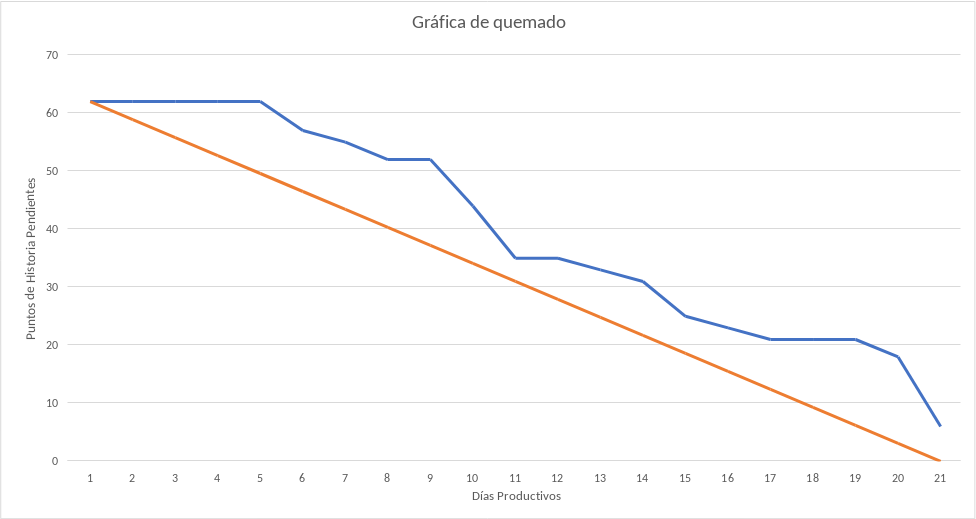
\includegraphics[height= 10cm, width=15cm]{project/images/graficoQuemado.png}
  \caption{\textbf{Gráfica de quemado}}
\end{figure}